%!TEX root=paper.tex

\section{Grouping Requests}
\label{sec:user}

For service endpoints which run computations in real time, the maintainer of a system might want to understand the endpoint performance on a per-user basis, especially for situations where the system response time is a function of some individual user load\footnote{E.g. in GMail some users have two emails while other have twenty thousand and this induces different response times for different users}.


To enable this, the \tool must be configured to associate an API call with a given user. The simplest way is to take advantage of the architecture of Flask applications in which a global \code{flask.request} object can be used to retrieve the session which can in turn lead to user identification: 

\begin{lstlisting}[style=custompython]  
# LOC #2: configure the dashboard
# to group requests by the user id
dashboard.config.group_by = 'User',
	lambda: Session.find(flask.request).user.id

\end{lstlisting}

Explain the code: the group by is assigned a tuple: 

\begin{itemize}
	\item 'User' stands for the name of the grouping
	\item the ``lambda'' stands for a function that takes as argument
	the global flask.request. Every application must have a way of
	associating a user with a request. Or an app with a request. 
	A user is usually retrieved from some session variable. 
	If we wanted to group by the user group for example, the code
	would change slightly by replacing ``user.id'' with ``user.group.id''
\end{itemize}

% \niceseparator

In Zeeguu, \epFeedItems retrieves a list of recommended articles for a given user. Cf. \Fref{fig:ep} it is the endpoint with the slowest response time and highest variability. The reason for this is that a user can be subscribed to anything from one to three dozen article sources and for each of the sources the system must compute the personalized difficulty of each article at every request. 


\begin{figure}[h!]
  \centering
  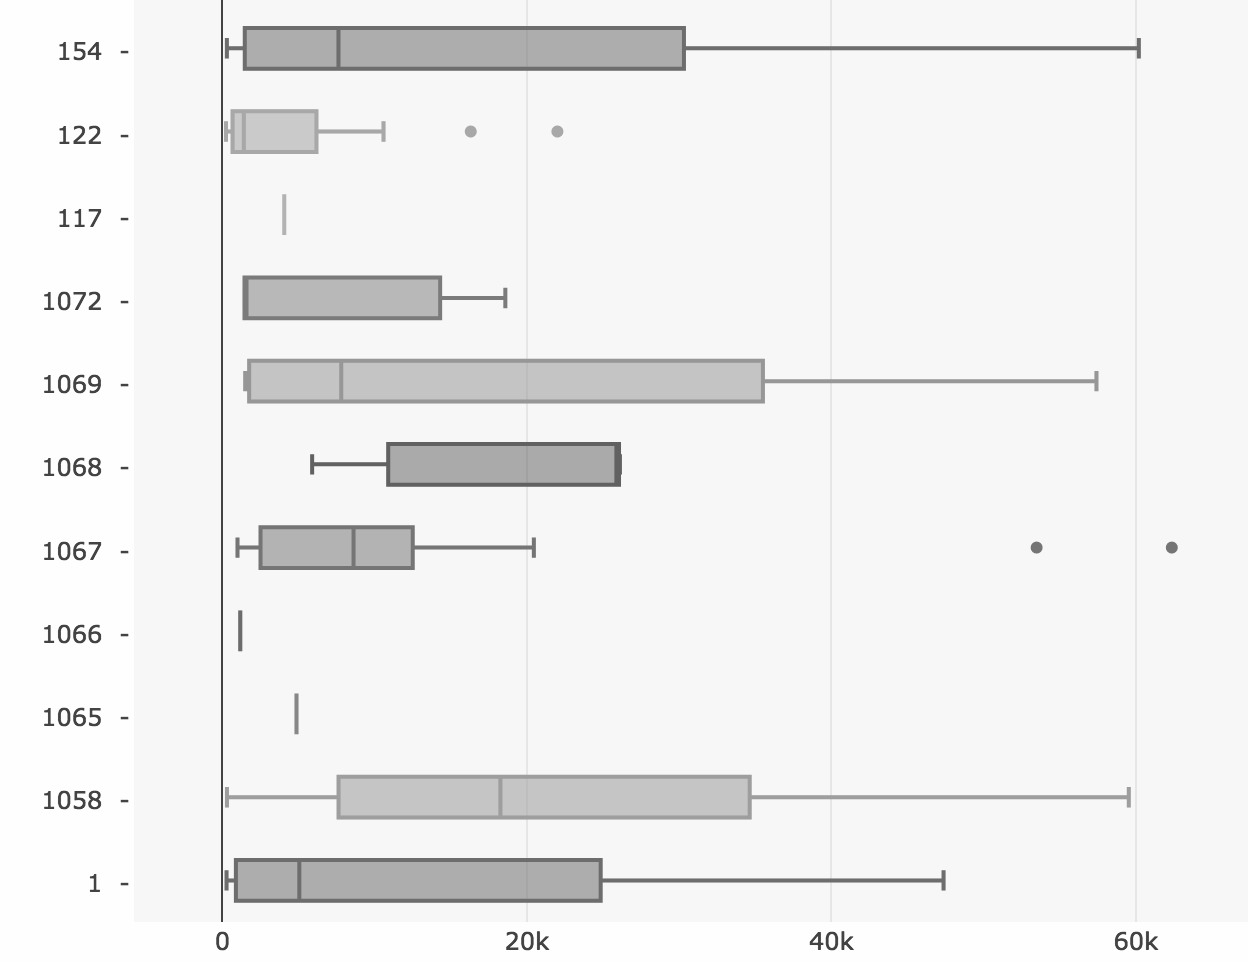
\includegraphics[width=.5\linewidth]{time_per_user}
  \caption{The \epFeedItems shows a very high variability across users}
  \label{fig:tpu}
\end{figure}


A \perspective{Per-User Performance} perspective should show the different response times for different users. Figure \ref{fig:tpu} presents a subset of the corresponding view in the \tool. The figure shows that the response times for this endpoint can vary considerably for different users with some extreme cases where a user has to wait a full minute until their recommended articles are shown\footnote{After seeing this perspective, the maintainer refactored the architecture of the system to move part the difficulty computation out of the interactive loop}.






